%%%%%%%%%%%%%%%%%%%%%%%%%%%%%%%%%%%%%%%%%%%%%%%%%%%%%%%%%%%%%%%%%%%%%%
%%%%%%%%%%%%%%%%%%%%%%%%%%%%%%%%%%%%%%%%%%%%%%%%%%%%%%%%%%%%%%%%%%%%%%
\documentclass[dvips,portrait]{seminar}             %%%%%%%%%%%%%%%%%%
                                                    %%%%%%%%%%%%%%%%%%
%%%%%%%%%%%%%%%%%%%%%%%%%%%%%%%%%%%%%%%%%%%%%%%%%%%%
% ./tex_to_ps KKquarks
% ./txp_to_eps tab1-189GeV
% ./txp_to_eps tab2-189GeV
% ./txp_to_eps tab1wt-189GeV
% ./txp_to_eps tab2wwt-189GeV
% pstops '1:0@0.925(10mm,-1mm)' KKquarks.ps  KKquarks-redu.ps
%======================

%%%%%%%%%%%%%%%%%%%%%%%%%%%%%%%%%%%%%%%%%%%%%%%%%%%%%%%
%%%%%%%%%%%%%%%%%%%%%%%%%%%%%%%%%%%%%%%%%%%%%%%%%%%%%%%
\begin{document}                     %%%%%%%%%%%%%%%%%%


\def\title{\Color{PineGreen} Quarks from \KK MC}

%%%%%%%%%%%%%%%%%%%%%%%%%%%%%%%%%%%%%%%%%%%%%%%%%%%%%%%%%%%%%%%%%%%%%%%%%%%%%
%%%%%%%%%%%%%%%%%%%%%%%%%%%%%%%%%%%%%%%%%%%%%%%%%%%%%%%%%%%%%%%%%%%%%%%%%%%%%
%%%%%%%%%%%%%%%%%%%%%%%%%%%%%%%%%%%%%%%%%%%%%%%%%%%%%%%%%%%%%%%%%%%%%%%%%%%%%
\begin{slide*}                                                %%%%%%%%%%%%%%%
\titbox{{\large\Color{Magenta} \KK MC versus \KK sem and KORALZ}}

{\bf\color{blue}
The aim of the following study is to check \KK MC 
for quark channels at LEP2. In particular:\\
(a) check agreement with semianalytical \KK sem, \\
(b) check differences with the KORALZ 4.02 and 4.04,\\
(c) compare runs with WTed events and WT=1 events,\\
(d) check the inclusive mode in \KK MC,\\
(e) provide a benchmark for the users of \KK MC.

\vspace{2mm}
Note that both \KK MC and KORALZ are run with vvmax=0.99 input parameter.\\
FSR is switched off.\\
No attempt to tune electroweak DIZET library --
the default EW setting of KORAZ and \KK MC is used.
}

\vfill
\end{slide*}   %%%
%%%%%%%%%%%%%%%%%%


%%%%%%%%%%%%%%%%%%%%%%%%%%%%%%%%%%%%%%%%%%%%%%%%%%%%%%%%%%%%%%%%%%%%%%%%%%%%%
%%%%%%%%%%%%%%%%%%%%%%%%%%%%%%%%%%%%%%%%%%%%%%%%%%%%%%%%%%%%%%%%%%%%%%%%%%%%%
%%%%%%%%%%%%%%%%%%%%%%%%%%%%%%%%%%%%%%%%%%%%%%%%%%%%%%%%%%%%%%%%%%%%%%%%%%%%%
\begin{slide*}                                                %%%%%%%%%%%%%%%
\titbox{{\large\Color{Magenta} \KK MC versus \KK sem, WT-ed events}}
{\large\bf\color{blue}
\noindent
Inclusive run of \KK MC, $q=d,u,s,c,b$. \\
Energy: $\sqrt{s}$= 189GeV. FSR is off.\\
The only cut $v=1-s'/s<v_{\max}$.
}
\vspace{-2mm}
\begin{center}
\setlength{\unitlength}{1mm}
\begin{picture}(70,60)
%#####\put(0,0){\framebox( 65,60){ }}
\put(0,0){\makebox(0,0)[lb]{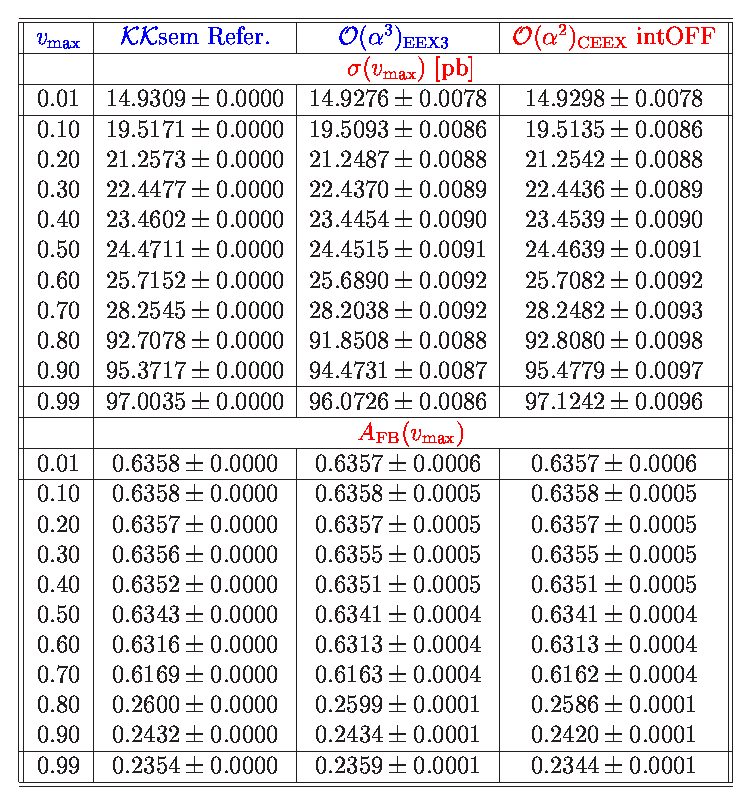
\epsfig{file=tab1wt-189GeV.eps,width=70mm,height=60mm}}}
\end{picture}
\end{center}
\vspace{1mm}
\noindent
{\large\bf\color{red}
 Satisfactory agreement   $<0.2\%$   for Z-excl. cuts.\\
 The same for Z-inclusive cuts.
}
\vfill
\end{slide*}   %%%
%%%%%%%%%%%%%%%%%%

%%%%%%%%%%%%%%%%%%%%%%%%%%%%%%%%%%%%%%%%%%%%%%%%%%%%%%%%%%%%%%%%%%%%%%%%%%%%%
%%%%%%%%%%%%%%%%%%%%%%%%%%%%%%%%%%%%%%%%%%%%%%%%%%%%%%%%%%%%%%%%%%%%%%%%%%%%%
%%%%%%%%%%%%%%%%%%%%%%%%%%%%%%%%%%%%%%%%%%%%%%%%%%%%%%%%%%%%%%%%%%%%%%%%%%%%%
\begin{slide*}
\titbox{{\large\Color{Magenta} \KK MC versus \KK sem, WT=1 events}}
{\large\bf\color{blue}
\noindent
Inclusive run of \KK MC, $q=d,u,s,c,b$. \\
Energy: $\sqrt{s}$= 189GeV. FSR is off.\\
The only cut $v=1-s'/s<v_{\max}$.
}
\vspace{-2mm}
\begin{center}
\setlength{\unitlength}{1mm}
\begin{picture}(70,60)
%#####\put(0,0){\framebox( 65,60){ }}
\put(0,0){\makebox(0,0)[lb]{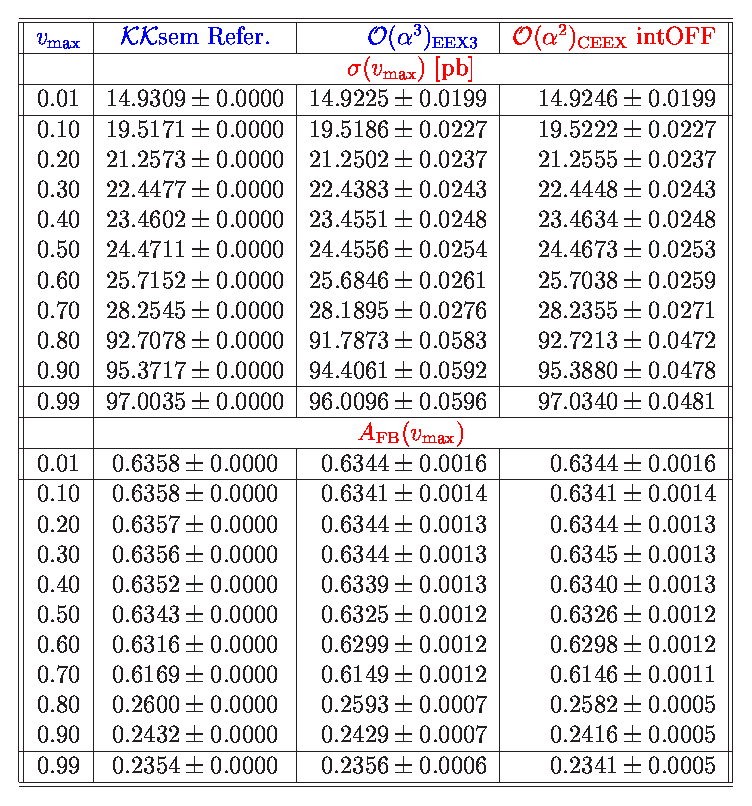
\epsfig{file=tab1-189GeV.eps,width=70mm,height=60mm}}}
\end{picture}
\end{center}
\vspace{1mm}
\noindent
{\large\bf\color{red}
 Satisfactory agreement   $<0.2\%$ for Z-excl. cuts.\\
 The same for Z-inclusive cuts.
}
\vfill
\end{slide*}   %%%
%%%%%%%%%%%%%%%%%%


%%%%%%%%%%%%%%%%%%%%%%%%%%%%%%%%%%%%%%%%%%%%%%%%%%%%%%%%%%%%%%%%%%%%%%%%%%%%
%%%%%%%%%%%%%%%%%%%%%%%%%%%%%%%%%%%%%%%%%%%%%%%%%%%%%%%%%%%%%%%%%%%%%%%%%%%%%
%%%%%%%%%%%%%%%%%%%%%%%%%%%%%%%%%%%%%%%%%%%%%%%%%%%%%%%%%%%%%%%%%%%%%%%%%%%%%
                                                         %%%%%%%%%%%%%%%%%%%%
\begin{slide*}
\titbox{{\large\Color{Magenta} \KK MC versus KORALZ 4.02 and 4.04}}
\noindent
{\large\bf\color{blue}
WT-ed events. $\sqrt{s}$= 189GeV. FSR is off.\\
\KK MC: inclusive run $q=d,u,s,c,b$. \\
The only cut $v=1-s'/s<v_{\max}$.
}
\begin{center}
\setlength{\unitlength}{1mm}
\begin{picture}(80,65)
%#####\put(0,0){\framebox( 65,60){ }}
\put(0,0){\makebox(0,0)[lb]{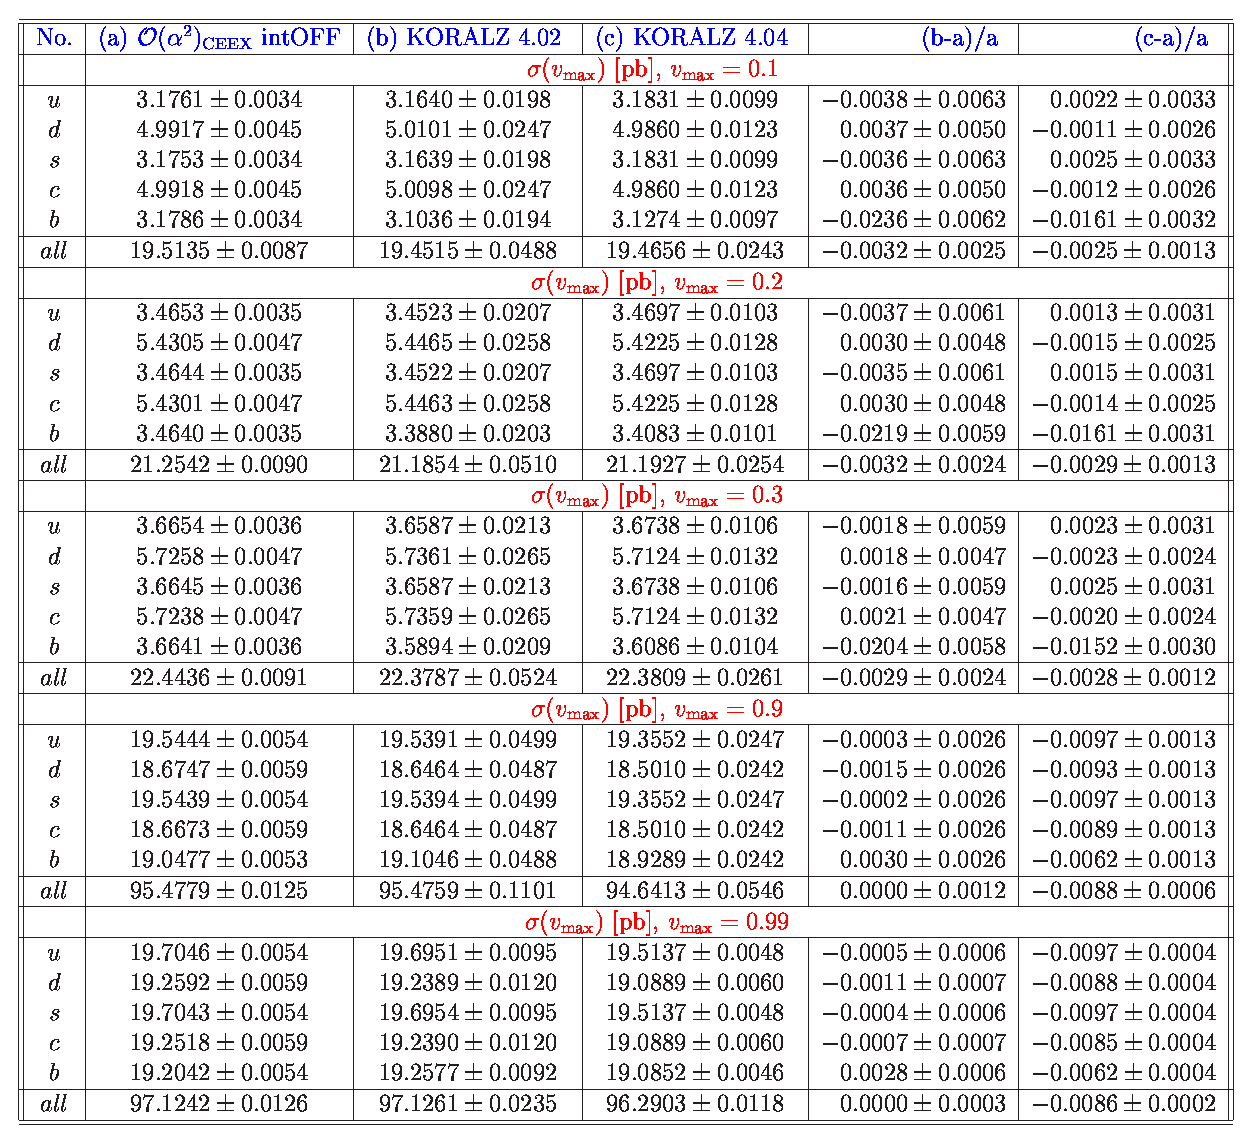
\epsfig{file=tab2wt-189GeV.eps,width=80mm,height=70mm}}}
\end{picture}
\end{center}
\vspace{-2mm}
\noindent
{\large\bf\color{red}
\KK MC agrees with KORALZ 4.02 and 4.04 generally better than 1\%, except $b$ quark.
}
\vfill
\end{slide*}   %%%
%%%%%%%%%%%%%%%%%%


%%%%%%%%%%%%%%%%%%%%%%%%%%%%%%%%%%%%%%%%%%%%%%%%%%%%%%%%%%%%%%%%%%%%%%%%%%%%
%%%%%%%%%%%%%%%%%%%%%%%%%%%%%%%%%%%%%%%%%%%%%%%%%%%%%%%%%%%%%%%%%%%%%%%%%%%%%
%%%%%%%%%%%%%%%%%%%%%%%%%%%%%%%%%%%%%%%%%%%%%%%%%%%%%%%%%%%%%%%%%%%%%%%%%%%%%
                                                         %%%%%%%%%%%%%%%%%%%%
\begin{slide*}
\titbox{{\large\Color{Magenta} \KK MC versus KORALZ 4.02 and 4.04}}
\noindent
{\large\bf\color{blue}
WT=1 events. $\sqrt{s}$= 189GeV. FSR is off.\\
\KK MC: inclusive run $q=d,u,s,c,b$. \\
The only cut $v=1-s'/s<v_{\max}$.
}
\begin{center}
\setlength{\unitlength}{1mm}
\begin{picture}(80,65)
%#####\put(0,0){\framebox( 65,60){ }}
\put(0,0){\makebox(0,0)[lb]{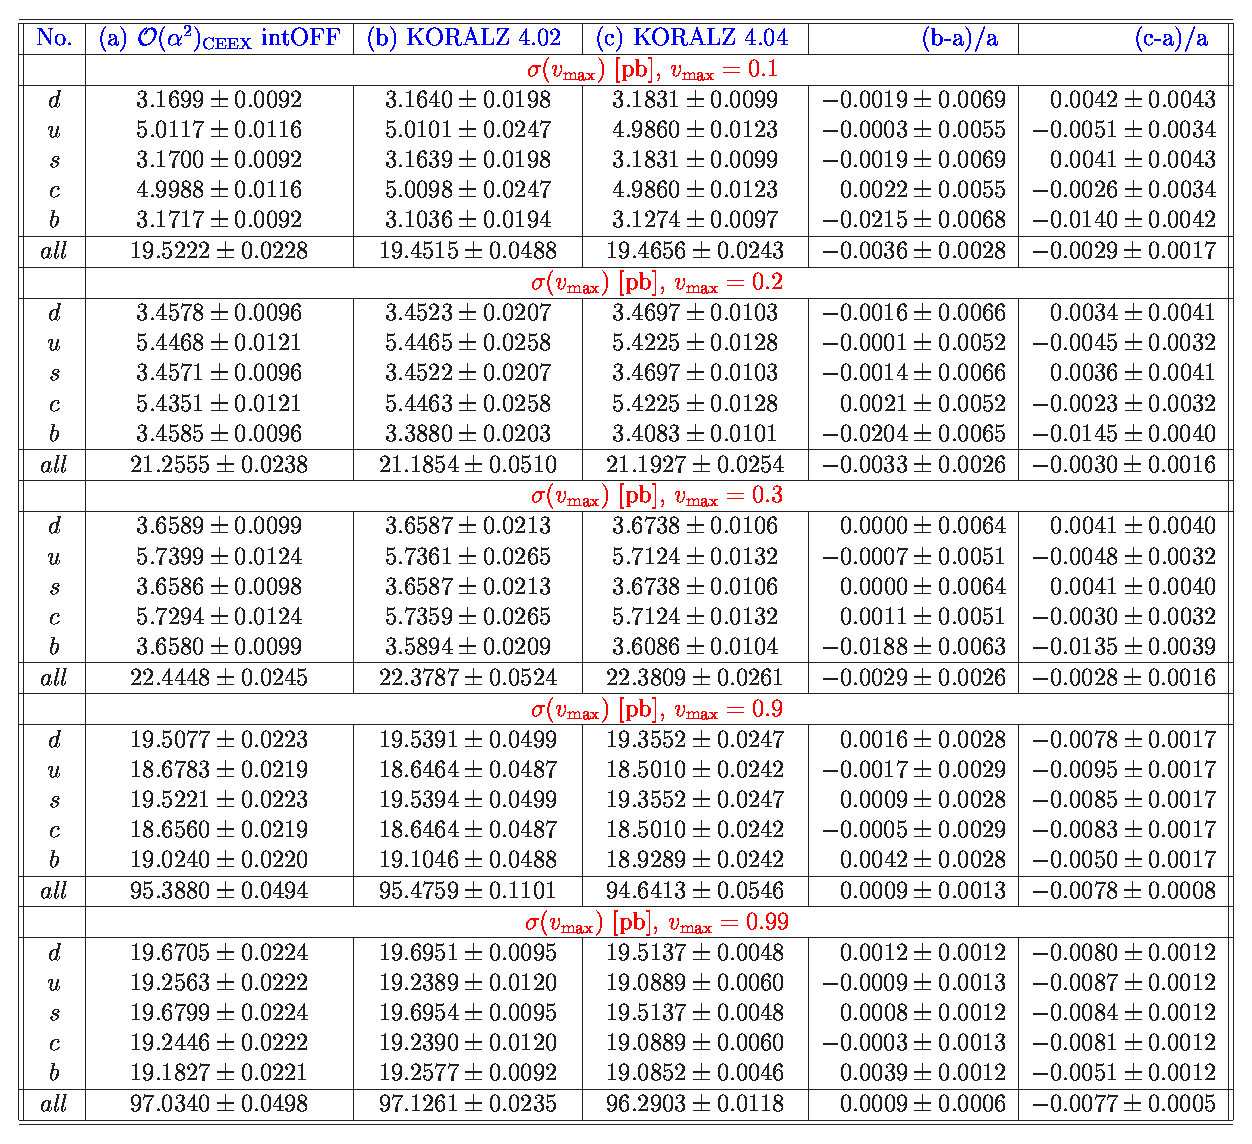
\epsfig{file=tab2-189GeV.eps,width=80mm,height=70mm}}}
\end{picture}
\end{center}
\vspace{-2mm}
\noindent
{\bf\color{red}
\KK MC agrees with KORALZ 4.02 and 4.04 generally better than 1\%.}
{\bf\color{red} Possible 1.5\% problem for $b$-quark?}
\vfill
\end{slide*}   %%%
%%%%%%%%%%%%%%%%%%


\end{document}

